\documentclass[compress, xelatex, 11pt, xcolor=dvipsnames, print, aspectratio=169,
	hyperref={
		bookmarks=true,
		unicode=true,
		colorlinks=true,
		pdftitle={Skautska vychovna metoda},
		plainpages=false,
		pdfauthor={Vojtech Zeisek},
		pdfsubject={Skautska vychovna metoda a jeji vyvoj za posledni stoleti a desetileti},
		pdfcreator={XeLaTeX},
		pdfkeywords={Junak, Pedagogika, Skaut, Skauting, Vychovna metoda},
		linkcolor=Red, % Navigační dokazy v menu na stránkách a v navigačních lištách
		anchorcolor=ForestGreen, % Nepoužívá se?
		citecolor=ForestGreen, % Nepoužívá se?
		filecolor=ForestGreen, % Nepoužívá se?
		menucolor=ForestGreen, % Nepoužívá se?
		urlcolor=Sepia, % Odkazy s \href a \url
		pdftex},
	url={hyphens, lowtilde} % Povolí řádkové zlomy v adresách
	]{beamer}

% Nastavení vzhledu

\usecolortheme{spruce}
\useinnertheme[shadow]{rounded}
\useoutertheme{shadow}

\setbeamertemplate{headline} {
	\hbox{%
		\begin{beamercolorbox}[wd=0.5\paperwidth, ht=2.65ex, dp=1.5ex, right]{section in head/foot}
			\insertsectionnavigationhorizontal{0.5\paperwidth}{\hskip0pt plus1fill}{\hskip0pt plus1fill}
			\end{beamercolorbox}%
		\begin{beamercolorbox}[wd=0.5\paperwidth, ht=2.65ex, dp=1.5ex, left]{subsection in head/foot}
			\insertsubsectionnavigationhorizontal{0.5\paperwidth}{}{\hfill\hfill}
			\end{beamercolorbox}%
		}
	\vskip 0pt
	}

\setbeamertemplate{footline} {
	\hbox{%
		\begin{beamercolorbox}[wd=0.3\paperwidth, ht=2.25ex, dp=1ex, center]{author in head/foot}
			\usebeamerfont{author in head/foot}\insertshortauthor~(\insertshortinstitute)
		\end{beamercolorbox}%
		\begin{beamercolorbox}[wd=0.4\paperwidth, ht=2.25ex, dp=1ex, center]{title in head/foot}
			\usebeamerfont{title in head/foot}\insertshorttitle
		\end{beamercolorbox}%
		\begin{beamercolorbox}[wd=0.3\paperwidth, ht=2.25ex, dp=1ex, right]{date in head/foot}
			\usebeamerfont{date in head/foot}\insertshortdate{}\hspace*{2em}
			\insertframenumber{}/\inserttotalframenumber\hspace*{2ex}
		\end{beamercolorbox}%
		}
	\vskip 0pt
	}

% Fonty Linux Libertine
\usepackage{libertine}

% Další balíčky
\usepackage{multicol}

% Jazyk
\usepackage[main=czech]{babel}

% Uvozovky
\usepackage[autostyle=true, czech=quotes]{csquotes}

% Úvodní stránka
\author{Vojtěch Zeisek}
\institute[Junák --- český skaut]{Ekologický odbor Výkonné rady Junáka --- českého skauta, z.~s.\\
Katedra botaniky Přírodovědecké fakulty UK \&~Botanický ústav AV ČR, v.~v.~i.\\
\href{mailto:zeisek@natur.cuni.cz}{zeisek@natur.cuni.cz}, \url{https://trapa.cz/cs}}
\title{Skautská výchovná metoda}
\subtitle{A~její vývoj za~poslední století a~desetiletí}
\titlegraphic{
\includegraphics[width=1.5cm]{lilie.png}}
\date{KDF MFF UK 27. 3. 2024}

% Prezentace
\begin{document}

\begin{frame}
	\titlepage
\end{frame}

\begin{frame}{Obsah}
	\begin{multicols}{2}
		\tableofcontents
	\end{multicols}
\end{frame}

\section{Úvod}

\subsection{Světová historie}

\begin{frame}{Jak to začalo --- velmi stručná historie světového skautingu}
	\begin{itemize}
		\item Skautské hnutí založil britský generál Robert Stephenson Smyth Baden-Powell, pozdější Lord of Gilwell, 1857--1941
		\item Nepřijat na~Oxford, 1876 nastupuje na~vojenskou akademii a~odjíždí do~Indie
		\item Kreslil, hrál divadlo, psal do~novin, učil se~hindsky, inspiruje se~místními stopaři a~zakládá průzkumné oddíly (anglicky \textit{scouts})
		\item 1887 připlouvá do~Jižní Afriky, převelen ke~zpravodajské službě, později inspektor jezdectva, mj. mapuje Dračí hory, \textbf{sepisuje příručku pro vojenské průzkumníky} (o~pohybu v~přírodě --- později inspirace pro děti pro pobyt v~přírodě),~\ldots
		\item 1899--1900 úspěšně brání obležený Mafeking před Búry, povýšen na~generálmajora, národní hrdina
		\item Žádá o~propuštění z~armády, \textbf{1907 1.~skautský tábor} (Brownsea Island), píše \textbf{Scouting for Boys} (1908)
		\item \textbf{1920 1.~světové Jamboree} (setkání) v~Londýně
	\end{itemize}
\end{frame}

\begin{frame}{Robert Baden-Powell (1857--1941)}{Co hlavního si pozdější mladý důstojník odnesl ze střední školy\ldots}
	\begin{center}
		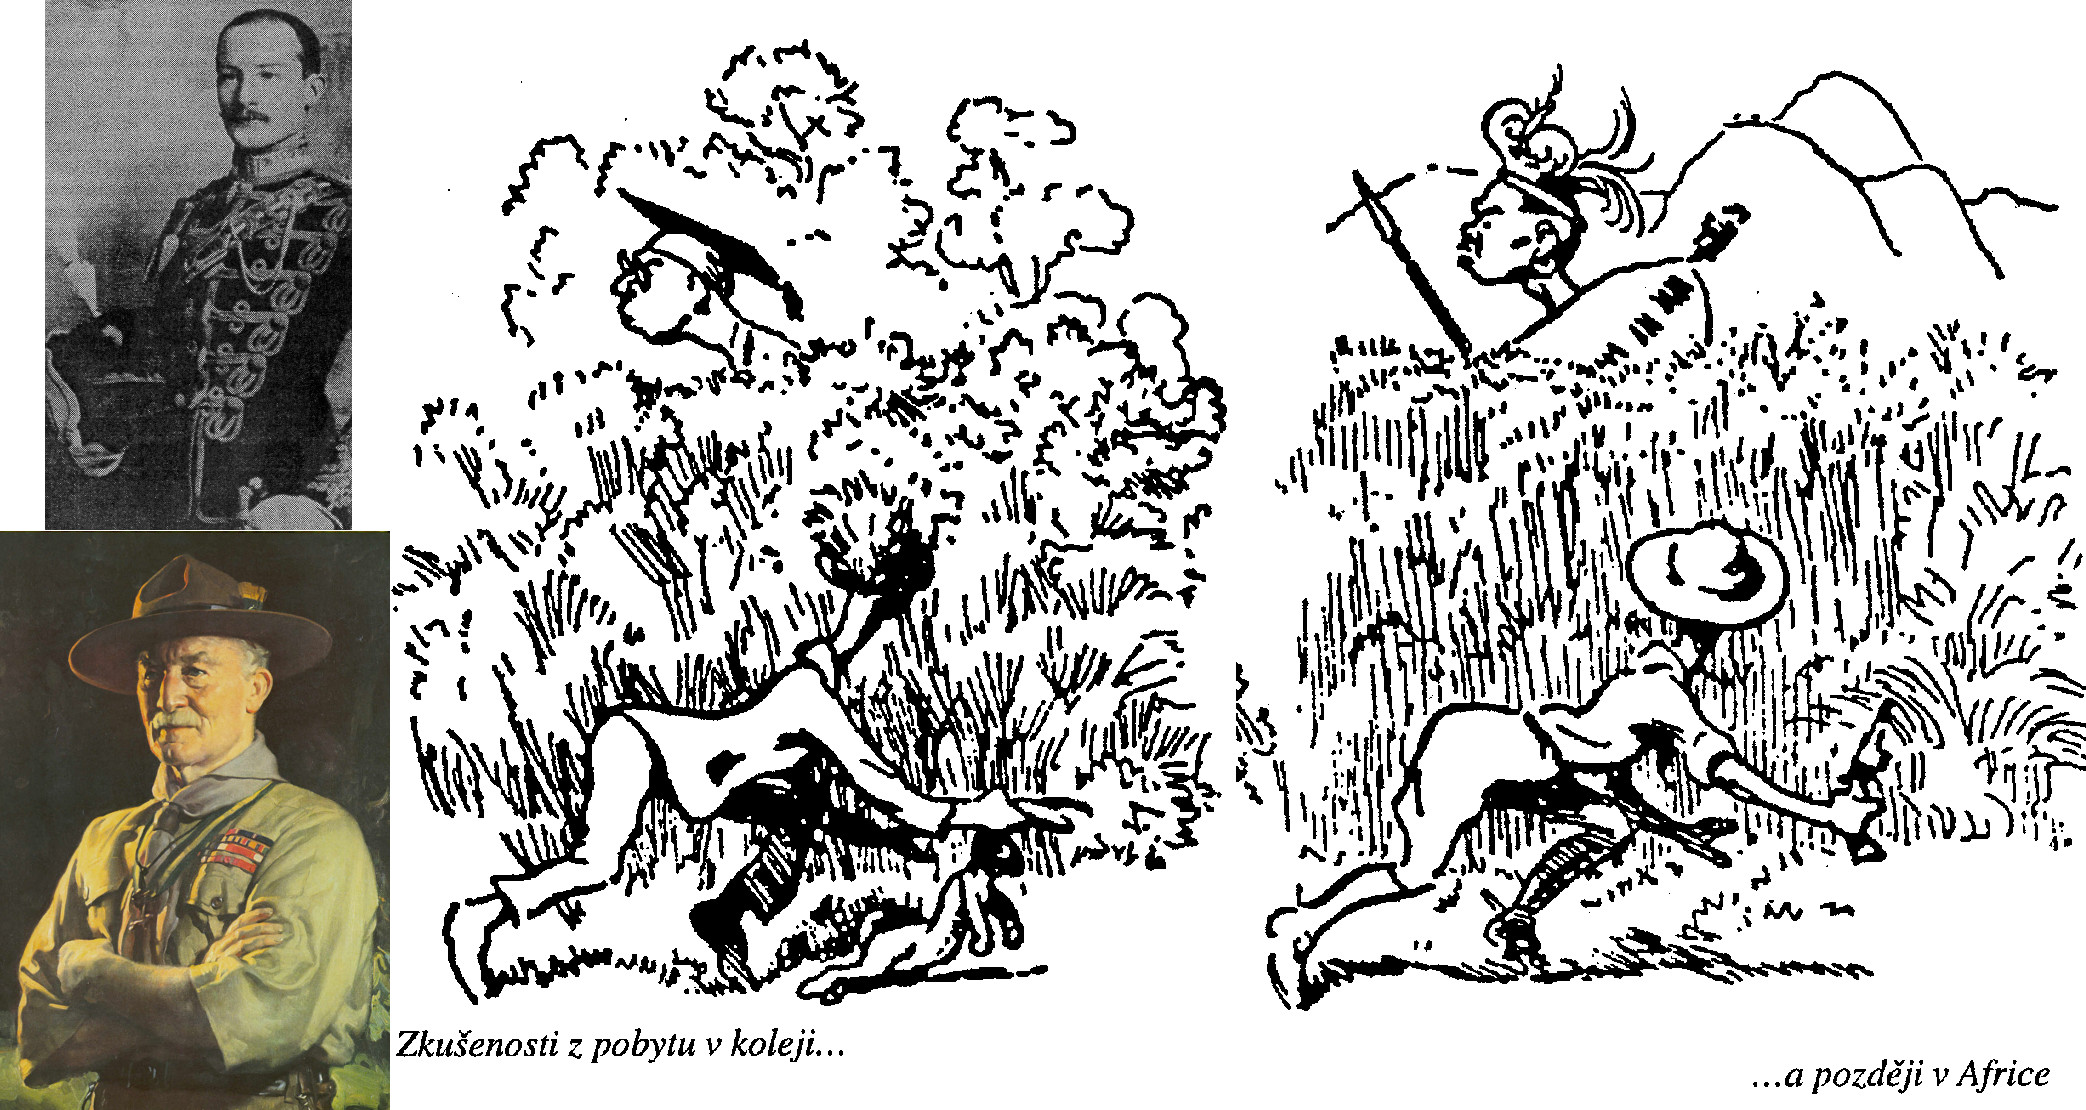
\includegraphics[height=6.5cm]{bp.jpg}
	\end{center}
\end{frame}

\begin{frame}{Ernest Thompson Seton (1860--1946)}{Woodcraft a~vliv na~český skauting I}
	\begin{multicols}{2}
		\begin{center}
			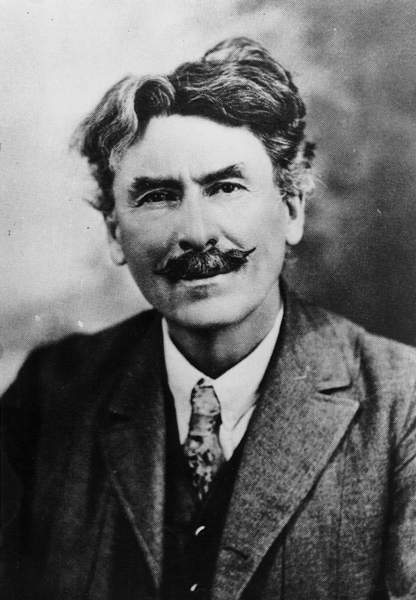
\includegraphics[height=6cm]{seton.jpg}
		\end{center}
		\columnbreak
		\begin{itemize}
			\item Původně anglický malíř, spisovatel, učitel a~přírodovědec
			\item Pracoval v~muzeu, živil se~i~psaním článků a~knih
			\item Skvělý pozorovatel a~vypravěč o~životě zvířat
			\item Většinu času trávil v~divoké přírodě v~USA, učil se~od~Indiánů jejich praktickým znalostem a~dovednostem i~filozofii, morálce a~pohledu na~svět
			\item Silná inspirace českého skautingu woodcraftem je světově unikátní
		\end{itemize}
	\end{multicols}
\end{frame}

\begin{frame}{Ernest Thompson Seton (1860--1946)}{Woodcraft a~vliv na~český skauting II}
	\begin{itemize}
		\item 1902 založil \textbf{Woodcraft Indians} --- hnutí inspirující se~životem Indiánů (ideou) a~snažící se~o~výchovu a~poznání
		\begin{itemize}
			\item Znalosti a~respekt k~přírodě
			\item Příroda a~krajina jako zdroj duchovní inspirace
			\item Fyzická zdatnost, rukodělné práce, zručnost
			\item Morální kodex
		\end{itemize}
		\item S~americkou skautskou organizací se~rozešel ve~zlém (\textit{Boy Scouts} pro něj byly příliš přísně organizované), s~Baden-Powellem vycházel velice dobře
		\item Trochu nespravedlivě ve~stínu skautingu, Woodcraft mnohem menší než skautské hnutí, vzájemně se~ovlivňovaly
		\item Mnoho společných prvků se~skautingem (práce v~malých skupinách, učení se~od~ostatních apod.), skauting klade větší důraz na~vztah ke~společnosti
		\item Knihy E.~T. Setona měly velký vliv na~zakladatele českého skautingu
		\item U~nás působí \href{https://www.woodcraft.cz/}{Liga lesní moudrosti} (přímo navazuje na~Setonovo americké hnutí)
	\end{itemize}
\end{frame}

\subsection{Česká historie}

\begin{frame}{Stručná historie českého skautingu I}
	\begin{itemize}
		\item \href{https://www.skaut.cz/skauting/historie/}{Junáka} založil pražský učitel tělocviku \textbf{Antonín \enquote{Benjamín} Svojsík}, 1876--1938
		\item 1909 se~dozvěděl o~skautingu, 1911 se~vydal do~Anglie
		\item \textbf{Ve školním roce 1911/12 založil na~žižkovské reálce 1.~skautskou družinu}, reakce veřejnosti byla chladná
		\item 1912 sepisuje \textbf{Základy junáctví}, konzultuje své myšlenky s~intelektuální elitou své doby (Drtina, Masaryk, Kramář, Aleš, Jirásek, Rais, Guth-Jarkovský,~\ldots)
		\item \textbf{1912 1. skautský tábor} u~Lipnice nad Sázavou (šli z~Prahy přes 100~km se~vším pěšky), přes celé prázdniny
		\item 1918 skauti pro revoluční Národní výbor zajišťovali kurýrní službu (a~vydávali 1.~známky Republiky Československé)
		\item 1919 založen Svaz junáků --- skautů RČS
		\item Vznikla řada skautských organizací (katoličtí, židovští,~\ldots)
		\item 1939 se~skautské organizace spojily do~Junáka --- svazu skautů a~skautek RČS
	\end{itemize}
\end{frame}

\begin{frame}{Antonín Benjamín Svojsík (1876--1938) a~první čeští skauti}
	\begin{itemize}
		\item Chtěl založit Junáka v~rámci Sokola, nakonec se~nedohodli
		\item Na přelomu 19. a~20. století vznikala řada podobných hnutí
	\end{itemize}
	\begin{center}
		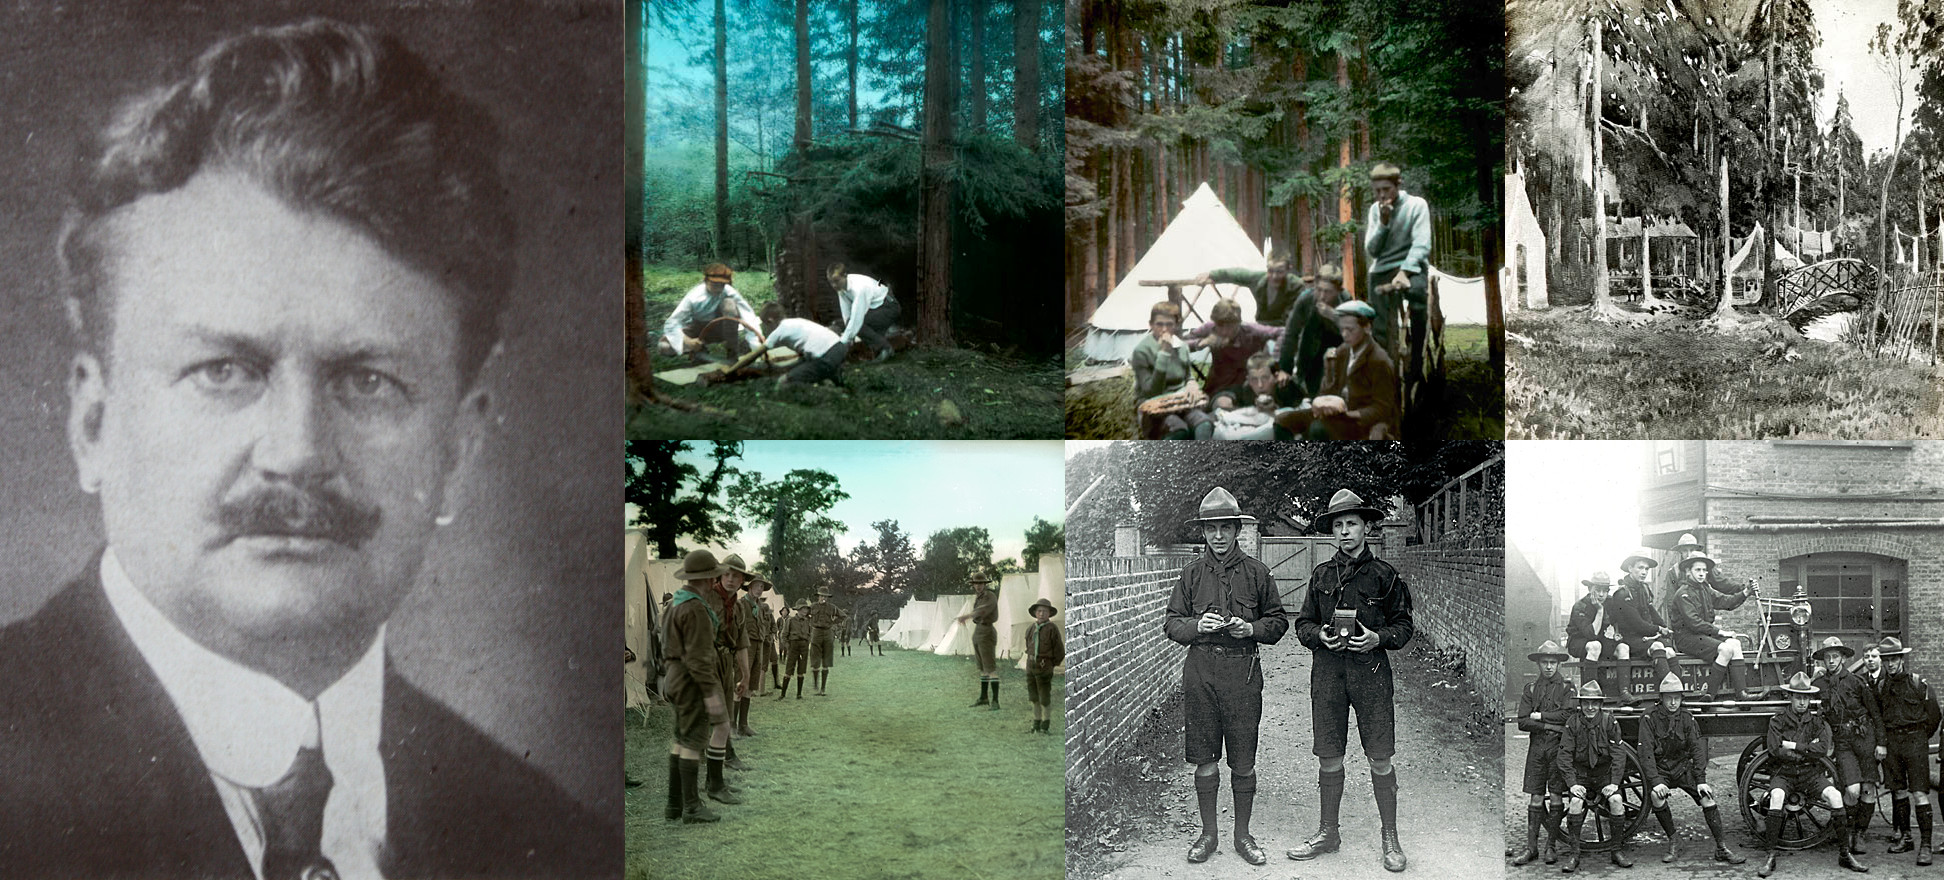
\includegraphics[height=5cm]{svojsik_prvni_skauti.jpg}
	\end{center}
	\begin{flushright}
		Kolorované fotografie z~tábora 1912, ostatní pravděpodobně z~20.~let
	\end{flushright}
\end{frame}

\begin{frame}{Stručná historie českého skautingu II}
	\begin{itemize}
		\item Přehled: \url{https://www.skautskyinstitut.cz/casova-osa}
		\item Za války se~skauti zapojili do~odboje, zahraničních armád (Zpravodajská brigáda byla největší (a~velmi úspěšná) odbojová organizace neodhalená Gestapem)
		\item 1940 Gestapo rozehnalo tábory, zatýkání představitelů, rozpuštění Junáka
		\item V~květnu 1945 se~skauti zapojili do povstání proti nacistům, Junák obnoven
		\item Ihned po únoru 1948 komunisti obsadili ústředí Junáka, vytvořen akční výbor, Junák zlikvidován
		\item 1949 měly vznikat pionýrské oddíly, 1950 Junák formálně zrušen (fakticky již neexistoval)
		\item V~50. letech bylo mnoho skautských činovníků odsouzeno za~protikomunistickou odbojovou činnost, někteří k~smrti
		\item 1968 Junák obnoven
		\item 1969 ÚV KSČ rozhodlo o~vzniku Svazu socialistické mládeže (SSM), 1970 Junák násilně včleněn do~SSM, fakticky zlikvidován
		\item V~70. a~80. letech řada oddílů přežívala pod hlavičkou jiných organizací v~rámci SSM
	\end{itemize}
\end{frame}

\begin{frame}{Junák od~90. let 20. století}
	\begin{itemize}
		\item 1989 obnova Junáka, raketový růst členů
		\item V~90. letech probíhaly debaty o~identitě a~budoucím směřování hnutí a~organizace
		\begin{itemize}
			\item Za totality měl každý svou představu, jak by měl vypadat skauting v~budoucí svobodné společnosti --- trvalo dlouho různé představy sjednotit\ldots
		\end{itemize}
		\item Výsledkem mnohdy bouřlivých debat byl mj. pokles počtu členů na~přelomu tisíciletí a~vznik dalších skautských organizací
		\item Počet členů Junáka nepřetržitě roste od~roku 2005 (\href{https://www.skaut.cz/skauting/fakta-a-cisla/}{nyní přes 76~000~členů a~téměř 2~300~oddílů})
		\item Díky zákazům během obou totalit nebyl čas na~vývoj programu a~reakce na~změny společnosti --- do~21. století jsme vstupovali prakticky s~programem z~30. let 20.~století\ldots
		\begin{itemize}
			\item Jak zachovat to dobré a~v~ostatním se~zmodernizovat?
			\item Co jsou klíčové prvky skautingu?
			\item Jak má vypadat současný skauting?
			\item Jasně vyplynula potřeba změny dosavadního programu
			\item \href{https://drive.google.com/file/d/1oq0Nz7ZnYIq6pac_f6G1oI8awuO9rjoz/view}{Charta českého skautingu (2005)}
		\end{itemize}
	\end{itemize}
\end{frame}

\subsection{Myšlenkové základy skautingu}

\begin{frame}{Poslání Junáka}{Globální cíl --- čeho chceme dosáhnout}
	\begin{center}
		\begin{Large}
			Posláním Junáka je \textbf{podporovat rozvoj osobnosti} mladých lidí, jejich \textbf{duchovních, mravních, intelektuálních, sociálních a~tělesných schopností} tak, aby byli po celý život připraveni plnit povinnosti k~sobě samým, bližním, vlasti, přírodě a~celému lidskému společenství \textbf{v~souladu s~principy a~metodami}, stanovenými zakladatelem skautského hnutí, lordem Robertem Baden-Powellem a~zakladatelem českého skautingu, prof. Antonínem Benjamínem Svojsíkem.
		\end{Large}
	\end{center}
	\begin{itemize}
		\item Za~1.~republiky se~na~tvorbě skautské metodiky podílely tehdejší špičky psychologie, pedagogiky a~dalších oborů
		\item Hledáme praktické a~atraktivní metody, jak toto poslání naplnit --- k~tomu slouží \textbf{výchovný program}
		\item Poslání je univerzální, naplňuje se~podle aktuálního stavu a~potřeb společnosti
	\end{itemize}
\end{frame}

\begin{frame}{Principy skautského hnutí}
	\begin{enumerate}
		\item \textbf{Povinnost k~Bohu}, chápaná jako povinnost hledat v~životě \textbf{vyšší hodnoty než materiální};
		\begin{itemize}
			\item Jde o~morálku, slušnost, dobrotu --- ne nutně o~víru
			\item Skauting je otevřený věřícím různých denominací i~ateistům
		\end{itemize}
		\item \textbf{povinnost vůči ostatním}, chápaná jako věrnost své vlasti, která je v~souladu s~úsilím o~mír, o~vzájemné pochopení a~spolupráci mezi lidmi, národy a~různými sociálními skupinami; je pojata jako \textbf{závazek účastnit se~na~rozvoji společnosti, jako úcta a~láska prokazovaná bližním a~přírodě};
		\begin{itemize}
			\item Nejsme tu jen sami za~sebe, ale jsme součástí širšího společenství, na~jehož běhu se~chceme aktivně podílet, díky své moci máme (jako lidé) zodpovědnost za~osud světa
		\end{itemize}
		\item \textbf{povinnost vůči sobě}, chápaná jako odpovědnost za~\textbf{rozvoj sebe sama}.
		\begin{itemize}
			\item Nesmíme zapomínat ani na~sebe (včetně odpočinku:-)
		\end{itemize}
	\end{enumerate}
	\vfill
	\begin{itemize}
		\item Principy musí být v~rovnováze, jakýkoliv nesmí převažovat
		\item Skautská výchovná metoda a~program hledá, jak principy prakticky naplnit
	\end{itemize}
\end{frame}

\begin{frame}{Skautský slib a~zákon}
	\begin{multicols}{3}
		\vfill
		\textbf{Slib}
		\vfill
		Slibuji na~svou čest, jak dovedu nejlépe: sloužit nejvyšší Pravdě a~Lásce věrně v~každé době, plnit povinnosti vlastní a~zachovávat zákony skautské, duší i~tělem být připraven pomáhat vlasti i~bližním.
		\vfill
		\textit{Dodatek pro věřící:} K~tomu mi dopomáhej Bůh.
		\vfill
		\textbf{Heslo}
		\vfill
		Buď připraven!
		\vfill
		\textbf{Zákon}
		\vfill
		Skaut je
		\begin{enumerate}
			\item pravdomluvný,
			\item věrný a~oddaný,
			\item prospěšný a~pomáhá jiným,
			\item přítelem všech lidí dobré vůle a~bratrem každého skauta,
			\item zdvořilý,
			\item ochráncem přírody a~cenných výtvorů lidských,
			\item poslušný rodičů, představených a~vůdců,
			\item veselé mysli,
			\item hospodárný,
			\item čistý ve~slovech, myšlení a~skutcích.
		\end{enumerate}
	\end{multicols}
\end{frame}

\begin{frame}{Cíl skautské výchovy}
	\begin{itemize}
		\item Základní vodítko: principy a~poslání skautského hnutí, skautský slib a~zákon
		\item \textbf{Výchovné cíle}
		\begin{itemize}
			\item Musí být v~souladu se~skautskými hodnotami (viz výše)
			\item Musí být praktické --- připravit děti na~reálný život
			\begin{itemize}
		\item Neznáme budoucnost --- co~bude \enquote{praktické} za~20--50 let?
			\end{itemize}
			\item Mohou jít proti mainstreamu --- masmédia,~\ldots
			\item Děti v~oddíle průměrně tráví pár hodin týdně na~schůzce, jednou za~pár týdnů den/víkend na~výpravě a~1--3~týdny na~táboře --- abychom je mohli pozitivně ovlivnit, musíme tento (oproti škole a~rodině) krátký čas využít maximálně efektivně
		\end{itemize}
		\item Musí to děti bavit
			\begin{itemize}
		\item \enquote{Ryby je nutné lovit na~to, co~chutná rybám a~ne na~to, co~chutná rybáři.} (Baden-Powell)
			\end{itemize}
		\item \textbf{Tvrdíme, že máme morální právo ovlivňovat hodnotový žebříček dětí směrem, který považujeme za~správný}
	\end{itemize}
\end{frame}

\begin{frame}{Povšimněte si\ldots}
	\begin{itemize}
		\item Zatím jsme neřekli nic o~\textit{konkrétní} programové náplni
		\item Skauting je definován \enquote{měkkými} cíly, ne konkrétními činnostmi --- na~rozdíl třeba od~sportovních klubů, tematických kroužků, apod.
		\item Veřejnost vnímá skauting převážně skrz táboření a~přírodu, ale to je (do~jisté míry) \enquote{jen} výchovný prostředek (viz dále)
		\item Mezi skautskými oddíly je obrovská tematická variabilita --- vodní, suchozemské, inspirující se~v~historii, věnující se~do hloubky nějakému oboru,~\ldots
		\item V~činnosti se~liší oddíly čistě dívčí, čistě chlapecké, smíšené; vlčácké, skautské a~roverské; z~vesnic a~z~velkých měst\ldots
		\item \ldots všem je společný stejný \alert{cíl}: \textbf{vychovat mladého člověka, který bude platným členem společnosti a~bude mít praktické schopnosti a~dovednosti pro život v~měnícím se~světě, za~jehož osud cítí (spolu)zodpovědnost a~podle toho jedná v~souladu s~morálními zásadami}
	\end{itemize}
\end{frame}

\section{Metodika}

\subsection{Výchovná metoda}

\begin{frame}{Skautská výchovná metoda\ldots}
	\ldots vede mladého člověka na~cestě osobního růstu: soustava výchovy a~sebevýchovy vedoucí k~upevňování charakteru, tvorbě hodnotového systému a~rozvoji dovedností a~znalostí:
	\begin{itemize}
		\item \textbf{Slib a~zákon} --- sebevýchova, dobrovolný závazek
		\item \textbf{Učení se~zkušeností} --- praktická i~mravní výchova
		\item \textbf{Družina} --- schopnost být platným členem společenství, pracovat v~týmu
		\item \textbf{Symbolický rámec} --- přitažlivé, inspirující a~obohacující
		\item \textbf{Příroda} --- výchovné prostředí, předmět zájmu, ochrany (od~lokálního prostředí po~klima) i~citového a~duchovního rozvoje
		\item \textbf{Program osobního růstu} --- pestrý, přitažlivý program i~všestranný individuální rozvoj (s~ohledem na~potřeby konkrétního člověka)
		\item \textbf{Dospělí průvodci} --- dospělí ukazují cestu, pomáhají, podporují a~povzbuzují s~respektem k~jedinečnosti dítěte
		\item \textbf{Zapojení do~společnosti} --- spolupráce s~místní komunitou
	\end{itemize}
	Definovaná \href{https://krizovatka.skaut.cz/spisovna/stanovy-junaka-ceskeho-skauta}{ve~stanovách}, \href{https://krizovatka.skaut.cz/vedu-oddil/skautska-vychova/skautska-vychovna-metoda}{\textbf{podrobně popsaná}} a~\href{https://krizovatka.skaut.cz/vedu-oddil/skautska-vychova}{rozpracovaná}.
\end{frame}

\begin{frame}{Historické podoby skautské výchovné metody I}
	\begin{multicols}{2}
		\textit{Základy junáctví}, Svojsík, 1912, 1921, reprint 1991
		\begin{itemize}
			\item Pobyt v~přírodě
			\item Umění pozorovati
			\item Táboření
			\item Noclehování v~přírodě
			\item Škola práce a~rytířství
			\item Fyzický vývoj a~vliv organizace
			\item (Vycházel ze \textit{Scouting for Boys} (Baden-Powell, 1908, česky 2009, \textit{Skauting pro chlapce}), knih Setona a~českých specifik)
		\end{itemize}
		\columnbreak
		\textit{Aids to Scoutmastership}, Baden-Powell, 1920, česky 2006 (\textit{Na pomoc skautským vůdcům})
		\begin{itemize}
			\item Charakterové vlastnosti
			\item Zdraví a~zdatnost
			\item Rukodělné práce a~řemeslné dovednosti
			\item Služba druhým
		\end{itemize}
		\begin{center}
			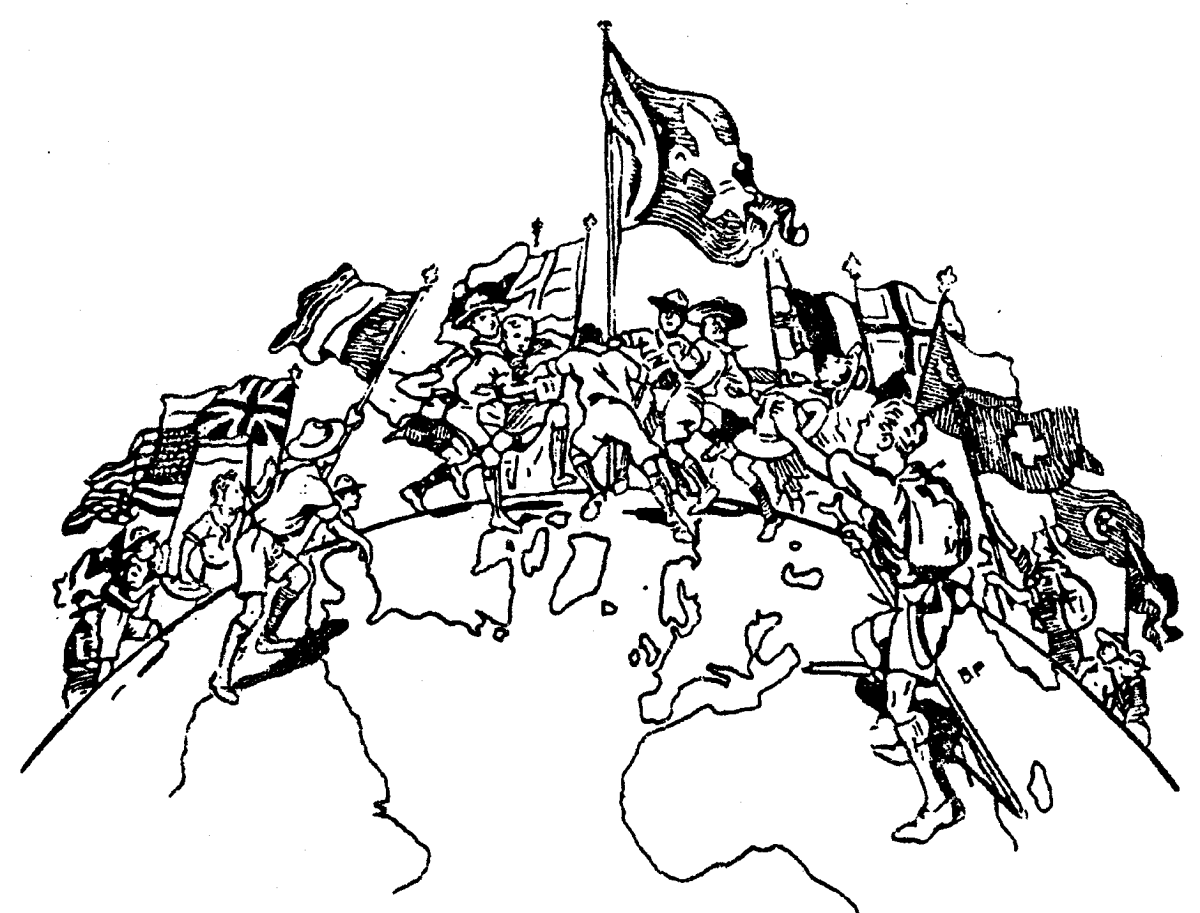
\includegraphics[width=2.5cm]{sireni.png}
		\end{center}
	\end{multicols}
\end{frame}

\begin{frame}{Historické podoby skautské výchovné metody II}
	\begin{multicols}{2}
		\textbf{WOSM}, 1977
		\begin{itemize}
			\item Slib a~zákon
			\item Učení se~zkušeností
			\item Členství v~malých skupinách
			\item Postupný a~stimulující program
		\end{itemize}
		\columnbreak
		\begin{scriptsize}
			\begin{itemize}
				\item World Organisation of Scout Movement
				\item World Association of Girl Guides and Girl Scouts
				\item International Scouts and Guide Fellowship
			\end{itemize}
		\end{scriptsize}
		\begin{center}
			
\includegraphics[height=1.75cm]{loga.png}
		\end{center}
	\end{multicols}
	\begin{itemize}
		\item Současná podoba české skautské výchovné metody \href{https://www.scout.org/who-we-are/scout-movement/scout-method}{odpovídá WOSM}
		\item Za~více jak 100~let se~metodika zásadně nezměnila --- posouval se~důraz a~detailnost formulace některých bodů
		\item \href{https://www.scout.org/}{WOSM} sdružuje skauty i~skautky, \href{https://www.wagggs.org/}{WAGGGS} jen skautky (hlavně v~rozvojovém světě řeší hodně ženská témata; některé země neumožňují registrace chlapců i~dívek ve~stejné organizaci), \href{http://www.isgf.org/}{ISGF} dospělé --- jejich metodiky se~zásadně neliší
	\end{itemize}
\end{frame}

\subsection{Čas na~změnu}

\begin{frame}{Proč nový program po roce 2000?}
	\begin{itemize}
		\item Změna společnosti
		\begin{itemize}
			\item Konzum, zrychlená doba, vliv médií, internetu, techniky,~\ldots
			\item Děti rychleji dospívají a~baví je jiné věci, než v~minulosti
		\end{itemize}
		\item Historický vývoj (zákazy,~\ldots) --- od~1. republiky do~přelomu tisíciletí se~moc nezměnil
		\item V~hnutí byla patrná nespokojenost se~stavem programu
		\item Charta českého skautingu (2005) --- obecné cíle rozvoje --- odkazuje na~historické kořeny, uvědomuje si současný svět a~otevírá skauting pro budoucnost
		\item Inspirace u~skautských organizací, které si podobným procesem prošly dříve (Irsko, Slovensko,~\ldots)
	\end{itemize}
	\begin{center}
		\begin{tabular}{ll}
			\textbf{\enquote{Starý program}} & \textbf{\enquote{Nový program}}\\
			Jednotlivé dílčí úkoly. & Komplexní úkoly, projekty.\\
			Hlavně o~znalostech. & Něco dokázat, udělat.\\
			Stejná úroveň pro všechny. & Nastavitelná obtížnost.\\
			Bez kontextu a~návaznosti. & Provázaný, motivační, atraktivní.
		\end{tabular}
	\end{center}
\end{frame}

\subsection{Program}

\begin{frame}{Výchovné kategorie}{Každá má svá specifika}
	\begin{itemize}
		\item \href{https://krizovatka.skaut.cz/benjaminci}{Benjamínci} --- předškolní děti
		\item \href{https://krizovatka.skaut.cz/svetlusky-zabicky-vlcata}{Světlušky, žabičky a~vlčata} --- mladší školní věk (cca 1. stupeň ZŠ)
		\item \href{https://krizovatka.skaut.cz/skautky-skauti}{Skautky a~skauti} --- starší školní věk (cca 2. stupeň ZŠ)
		\item \href{https://krizovatka.skaut.cz/roveri-rangers}{Rangers a~roveři} --- cca střední škola, počátek vysoké
		\item \href{https://krizovatka.skaut.cz/kmen-dospelych-a-rodinny-skauting/rodinny-skauting}{Rodinný skauting} --- tábory (bývalých) vedoucích s~(vlastními) malými dětmi
		\item \href{https://krizovatka.skaut.cz/kmen-dospelych-a-rodinny-skauting/kmen-dospelych}{Oldskauti} --- dospělí (nepůsobící přímo u~oddílů)
		\item Napříč výchovnými kategoriemi\ldots
		\begin{itemize}
			\item \href{https://casopis.skauting.cz/o-skautingu-pro-vsechny-9852}{Skauting pro všechny} --- jakkoliv znevýhodněné děti (zdravotní postižení,~\ldots)
			\item Průřezová témata jako \href{https://krizovatka.skaut.cz/organizace/ustredni-organy/odbory-vykonne-rady/skauti-na-zemi}{Skauti} \href{https://www.skautinazemi.cz/}{Na Zemi} (globální výchova), \href{https://krizovatka.skaut.cz/organizace/ustredni-organy/odbory-vykonne-rady/ekologicky-odbor}{ekologická výchova}, \href{https://krizovatka.skaut.cz/organizace/ustredni-organy/odbory-vykonne-rady/odbor-duchovni-vychovy}{duchovní výchova}, \href{https://krizovatka.skaut.cz/mezinarodni-skauting/zahranicni-odbor-and-international-tym}{zahraniční akce},~\ldots
			\item Učení se~(metodami vhodnými pro danou věkovou kategorii) zdravovědě, táboření, zručnosti, \enquote{soft skills},~\ldots
			\item Ve~všem co~děláme musíme mít na~paměti a~naplňovat poslání Junáka
		\end{itemize}
	\end{itemize}
\end{frame}

\begin{frame}{Výchovný program}
	\begin{itemize}
		\item Výsledek skautské výchovy --- výchovné cíle skautingu
		\begin{itemize}
			\item Mladý člověk cca na~konci střední až počátku vysoké školy
			\item Dovednosti, schopnosti a~postoje, které má mladý člověk ovládat --- koho chceme vychovat
		\end{itemize}
		\item Výchovné nástroje
		\begin{itemize}
			\item Skautská metoda
			\item Věkové kategorie
			\item \href{https://casopisy.skaut.cz/knihovna/r/metodika}{Metodické příručky pro vedoucí}, \href{https://casopisy.skaut.cz/}{časopisy},~\ldots
			\item \href{https://krizovatka.skaut.cz/fungujici-tym/zpetna-vazba-je-dulezita}{Hodnocení kvality} oddílu a~výchovného dopadu
			\item Podpora vedoucích a~dalších dospělých dobrovolníků --- management, \href{https://krizovatka.skaut.cz/organizace/ustredni-organy/odbory-vykonne-rady/odbor-pro-personalistiku}{lidské zdroje}, technická podpora (\href{https://krizovatka.skaut.cz/organizace/ustredni-organy/odbory-vykonne-rady/infoodbor}{IT},~\ldots), found rising, \href{https://krizovatka.skaut.cz/skautske-benefity}{benefity},~\ldots
			\item A~mnohé další\ldots
		\end{itemize}
		\item Velká reforma výchovného programu 2005--2013
		\begin{itemize}
			\item Vlastně nikdy nekončí\ldots
			\item Od podzimu 2016 jeho vyhodnocení a~začátek prací na~úpravách\ldots
		\end{itemize}
		\item Stále je dost práce\ldots
	\end{itemize}
\end{frame}

\begin{frame}{Jak při tvorbě výchovného programu postupujeme}
	\begin{enumerate}
		\item Definování obecných cílů (kompetence)
		\item Rozpracování dílčích cílů (podle věku,~\ldots)
		\item Výběr vhodných indikátorů (jak poznáme je-li cíl splněn) --- \enquote{projevy}
		\item Tvorba programů vedoucích ke~splnění cílů
	\end{enumerate}
	\begin{itemize}
		\item Body \textbf{3} a~zvláště \textbf{4} mohou mít velmi různou podobu
		\item Obecné cíle se~definovaly na~začátku pro všechny věkové kategorie
		\item Rozpracování obecných cílů se~provádí pro jednotlivé věkové kategorie (dílčí cíle)
		\item Další nástroje sloužící k~motivaci,~\ldots
		\item Postupná tvorba \href{https://chystamprogram.skaut.cz/}{databáze programů}
		\item Metodická podpora pro vedoucí a~další \enquote{uživatelská} podpora vedoucím oddílů ze~strany organizace (semináře, literatura,~\ldots)
		\item Výchovné nástroje jsou testovány, jejich funkčnost průběžně hodnocena
	\end{itemize}
\end{frame}

\begin{frame}{Co chceme, aby uměl mladý člověk poté, co~projde naší výchovou a~na~prahu dospělosti odejde?}
	\begin{center}
		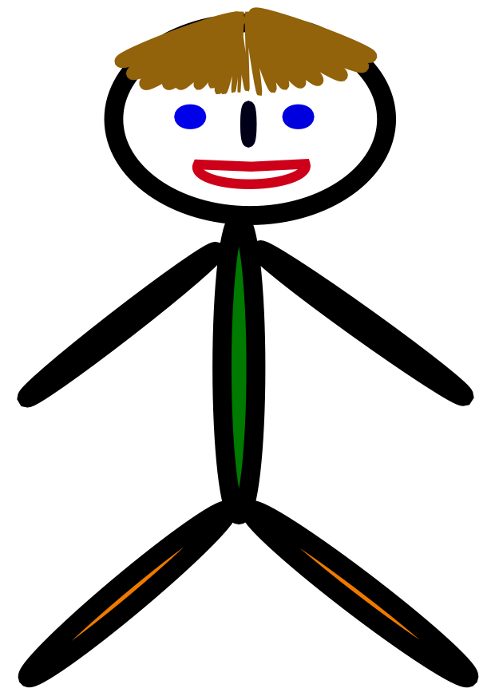
\includegraphics[height=6.25cm]{pepicek.png}
	\end{center}
\end{frame}

\subsection{Kompetence}

\begin{frame}{Skauting a~klíčové kompetence}
	\begin{center}
		Klíčové kompetence: přenosný a~univerzálně použitelný \textbf{soubor vědomostí, dovedností a~postojů}, které potřebuje každý jedinec \textbf{pro své osobní naplnění a~rozvoj, pro zapojení se~do~společnosti} a~úspěšnou zaměstnatelnost.
	\end{center}
	\begin{itemize}
		\item Kompetence je souborem schopností, dovedností, znalostí a~postojů vztahující se~k~určité oblasti
		\item Kompetence se~rovnají výchovným záměrům
		\item Jsou rozpracované pro jednotlivé kategorie
		\item Navazují na~ně výchovné cíle a~metody
		\item Úspěšnost definují indikátory (ukazatele, zda dochází k~rozvoji dané kompetence)
		\item Jsou zpracovávány a~konzultovány s~odborníky na~danou oblast (i~mimo Junáka)
		\item Vznikly po~mnoha diskuzích a~připomínkování (i~ze~strany oddílů)
		\item Od~2019 probíhá na~základě dosavadních zkušeností rozsáhlejší revize
	\end{itemize}
\end{frame}

\begin{frame}{Seznam kompetencí a~jejich podoblastí pro skautky a~skauty}
	\begin{enumerate}
		\item \textbf{Co umím a~znám} --- Praktický život; Fyzická zdatnost; Buď připraven; Hledání řešení; Tábornická praxe; Tvořivost a~zručnost
		\item \textbf{Kdo jsem} --- Já a~můj život; Moje svědomí; Osobní rozvoj
		\item \textbf{Moje kamarádství} --- Vztahy; Komunikace mezi lidmi, vyjadřování; Pomoc druhým
		\item \textbf{Můj domov} --- Moje rodina; Moje parta; Družina jako tým
		\item \textbf{Svět okolo nás} --- Já v~demokracii; Propojený svět; Rozmanitost světa; Příběhy našeho světa
		\item \textbf{Příroda kolem nás} --- Pobyt v~přírodě; Vnímání přírody; Poznávání přírody; Hodnota přírody; Šetrné chování
	\end{enumerate}
	\begin{itemize}
		\item Pro ostatní věkové kategorie se~podoblasti mírně liší
		\item Podrobně viz. \url{https://krizovatka.skaut.cz/vedu-oddil/skautska-vychova/k-cemu-vychovavame-aneb-kompetence-skautske-vychovy}
	\end{itemize}
\end{frame}

\begin{frame}{Příklad rozpracování jedné kompetence}
	\begin{itemize}
		\item Kompetence
		\begin{itemize}
			\item V~běžném životě se~zvládne postarat o~sebe i~ostatní. Umí řešit problémy, kriticky pracovat s~informacemi, učí se~z~řešení problému.
		\end{itemize}
		\item Výchovný cíl
		\begin{itemize}
			\item Umí uvařit sobě, rodině i~družině jídlo ze~základních surovin a~nakoupit k~tomu potřebné suroviny. (11--15 let)
		\end{itemize}
		\item Metody
		\begin{itemize}
			\item Nakupování potravin a~jiných věcí pro oddíl.
			\item Vedení pokladny družiny, vybírání peněz na~výpravě.
			\item Vaření na~výpravách.
		\end{itemize}
		\item Indikátory
		\begin{itemize}
			\item Šetří si nějaké peníze se~svého kapesného
			\item Nekupuje si zbytečnosti
			\item Bezchybně vrátí peníze po nákupu
		\end{itemize}
	\end{itemize}
	\alert{Smysl užívání kompetencí: \textbf{proměnit skautské principy v~život}}
\end{frame}

\section{Stezka}

\subsection{Struktura}

\begin{frame}{Stezka pro skautský věk}
	\begin{itemize}
		\item Jeden ze~základních výchovných nástrojů --- je všestranná, rozličná a~vyžaduje osobní zapojení vedoucích i~dětí
		\item \url{https://stezka.skaut.cz/}
	\end{itemize}
	\begin{center}
		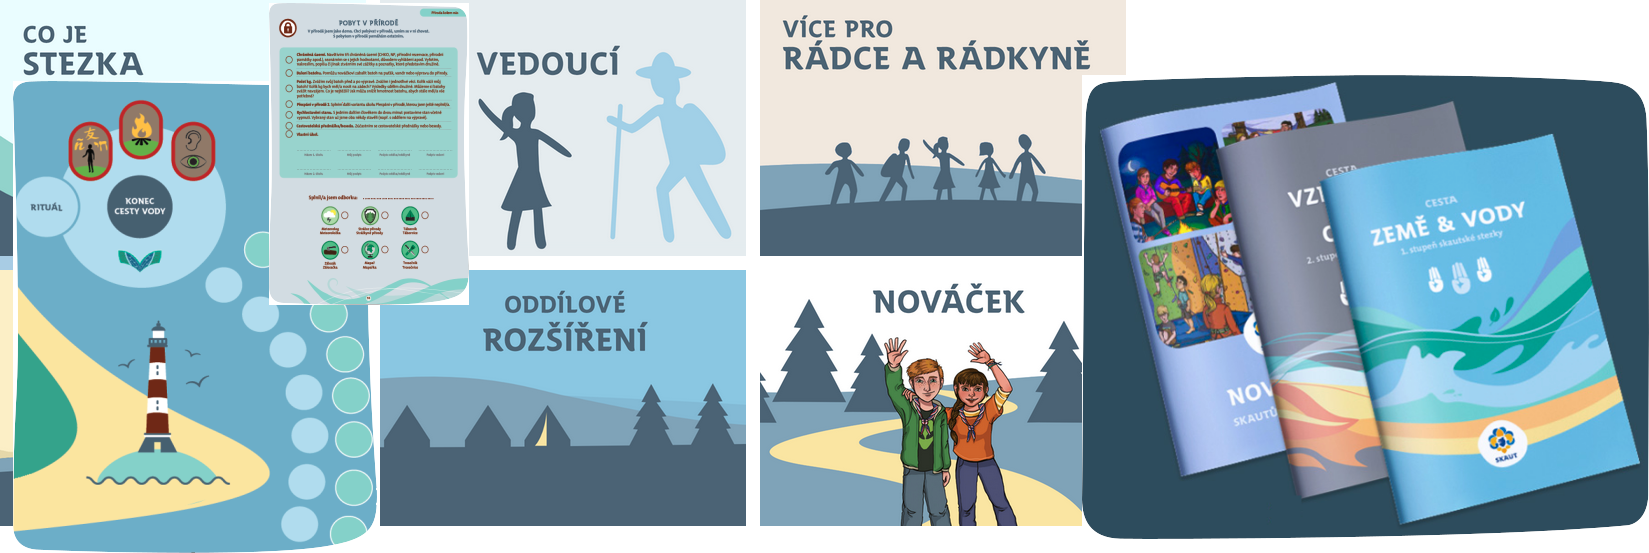
\includegraphics[width=\textwidth]{stezka.png}
	\end{center}
\end{frame}

\begin{frame}{Stezka není jen pár sešitů}
	\begin{multicols}{2}
		\begin{itemize}
			\item Propracovaný systém nástrojů a~motivace
			\item Prostředek k~dosahování výchovných cílů
			\item Hlavní průvodce na~cestě osobního rozvoje
			\item Nabízí zajímavý program
			\item Atraktivní a~srozumitelná forma
			\item Dva stupně, čtyři živly (Cesta Země \&~Vody, Cesta Vzduchu \&~Ohně)
			\item Ke stažení editovatelné \href{https://krizovatka.skaut.cz/skautky-skauti/stezky/ke-stazeni}{skautské} i~\href{https://krizovatka.skaut.cz/svetlusky-zabicky-vlcata/stezky-a-cesticky-vlcat-svetlusek-a-zabicek}{vlčácké} v~několika verzích
			\item Aktuálně zavádíme revidované verze
		\end{itemize}
		\columnbreak
		\begin{center}
			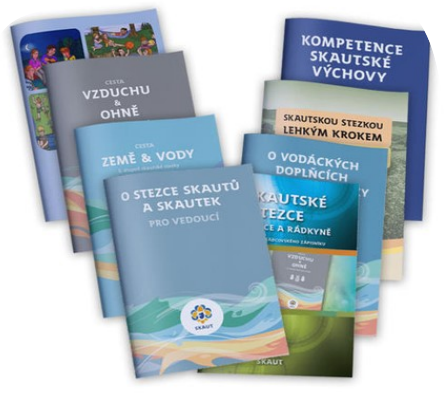
\includegraphics[height=6cm]{stezky.png}
		\end{center}
	\end{multicols}
\end{frame}

\subsection{Související nástroje}

\begin{frame}{Nováček --- pro začátek}
	\begin{multicols}{2}
		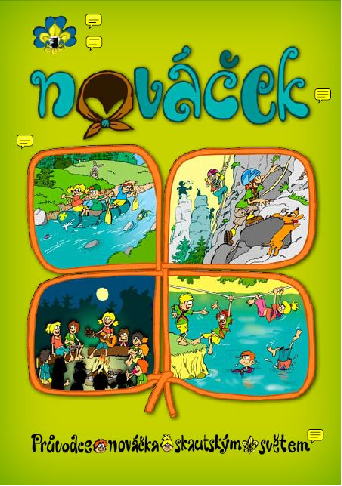
\includegraphics[height=6.5cm]{novacek.png}
		\columnbreak
		\begin{itemize}
			\item Uvede nováčka do~oddílu
			\item Zábavná forma
			\item Seznámí se~skautingem a~vším, co~k~němu patří
			\item Vodácké doplňky pro~vodní skauty
			\item Varianty pro světlušky, vlčata, skautky i~skauty
			\item Ke stažení \href{https://stezka.skaut.cz/novacek/}{skautské}, i~\href{https://krizovatka.skaut.cz/svetlusky-zabicky-vlcata/stezky-a-cesticky-vlcat-svetlusek-a-zabicek/2021-03/novacek-vlcat-svetlusek-a-zabicek}{vlčácké} v~různých variantách
			\item Oddíly si jej mohou upravit podle svých potřeb
		\end{itemize}
	\end{multicols}
\end{frame}

\begin{frame}{Pro roverský věk máme výzvy a~projekty}{Máme spoustu rozšiřujících metodických nástrojů\ldots}
	\begin{itemize}
		\item Roverská stezka
		\begin{itemize}
			\item Na~rozdíl od~mladšího věku není zásadním nástrojem, spíš doplňkem
			\item Vede k~rovnováze mezi jednotlivými oblastmi osobního rozvoje
			\item Vede k~hledání vnitřní motivace pro osobní rozvoj
			\item Odráží reálný život, nejen prostředí vlastní roverské skupiny či střediska
		\end{itemize}
		\item Výzvy a~projekty pro~rovery a~rangers
		\begin{itemize}
			\item Klíčové nástroje roverského programu
			\item Výběr plně v~rukou jednotlivých roverů a~rangers, případně celého roverského společenství
			\item R\&R by si je měli vybírat tak, aby se~rovnoměrně zaměřovali na~různé oblasti
		\end{itemize}
		\item Podrobněji \url{https://krizovatka.skaut.cz/roveri-rangers/roverska-stezka-vyzvy-a-projekty}
	\end{itemize}
\end{frame}

\begin{frame}{Odborky}
	\begin{itemize}
		\item Stezky pokrývají +/- společný základ, kterým by si (s~určitou individualizací) měli projít všichni
		\item Odborky reflektují šíři tématického záběru různých oddílů --- umožňují dětem rozvíjet se~v~nějaké oblasti (jsou vodítkem na~cestě k~určité odbornosti)
		\item Není účelem nahradit specializované kroužky, ale dát dětem prostor pro rozvoj individuálních zájmů
		\item Velký důraz je kladen na~sdílení znalostí s~oddílem --- vzájemné učení se
		\item Pro přehled viz \href{https://odborky.skaut.cz/}{skautské} a~\href{https://vlcciasvetylka.skaut.cz/}{vlčci a~světýlka pro světlušky, žabičky a~vlčata}; roveři a~rangers mohou \href{https://krizovatka.skaut.cz/roveri-rangers/odborky-pro-rovery-a-rangers}{plnit skautské}, ale i~tam působit jako mentoři
	\end{itemize}
	\begin{center}
		
\includegraphics[width=\textwidth]{odborky.jpg}
	\end{center}
\end{frame}

\begin{frame}{Stezka zdaleka není vše\ldots}{Některé nástroje fungují lépe, jiné hůře a~čekají je změny\ldots}
	\begin{itemize}
		\item Nováček (úvod do~oddílu a~skautingu), stezka a~další věci \url{https://stezka.skaut.cz/}
		\item Odborky \url{https://odborky.skaut.cz/} a~\url{https://vlcciasvetylka.skaut.cz/}
		\item Časopis Skaut \url{https://casopisy.skaut.cz/skaut/} a~\href{https://casopisy.skaut.cz/}{další}
		\item Svojsíkův závod \url{https://zavody.skaut.cz/}
		\item Rádcovský rozcestník \url{https://radce.skaut.cz/} pro vedoucí skautských družin
		\item A~\href{https://krizovatka.skaut.cz/vedu-oddil}{více}\ldots
	\end{itemize}
\end{frame}

\subsection{Práce se~stezkou}

\begin{frame}{Výhody stezky}
	\begin{itemize}
		\item Všestrannost, rozličnost a~osobní zapojení
		\item Stezka je vodítkem pro vytváření celoročního programu
		\item Stezka umožňuje snadné přizpůsobení oddílu
		\item Propracovaný nástroj osobního rozvoje
		\item Zatraktivnění programu
		\item Během historie skautingu měla a~má mnoho podob
	\end{itemize}
	\begin{center}
		
\includegraphics[height=4cm]{im-possible_m.png}
	\end{center}
\end{frame}

\begin{frame}{Pravidla a~plnění stezky}
	\begin{itemize}
		\item Výběr úkolů
		\begin{itemize}
			\item 1.~stupeň --- vše povinné, 2.~stupeň --- výběr ze~4~variant u~každého úkolu
			\item Vybírá se~po konzultaci s~vedoucím (neplní se~všechny)
			\item Lze je plnit v~libovolném pořadí
			\item Úkol lze upravit, vymyslet,~\ldots
		\end{itemize}
		\item Kdo hodnotí
		\begin{itemize}
			\item Dítě a~dvě další osoby (vedoucí, rádce, rodič, externí odborník,~\ldots)
		\end{itemize}
		\item Hodnocení
		\begin{itemize}
			\item Musí se~shodnout dítě a~další hodnotitel(é)
		\end{itemize}
		\item Plnění
		\begin{itemize}
			\item Přímé plnění
			\item Nepřímé plnění
			\item Přímé plnění s~přípravou
			\item Pro některé body nejsou vhodné všechny způsoby
		\end{itemize}
	\end{itemize}
\end{frame}

\section{Revize}

\subsection{Popis stavu, jeho zhodnocení}

\begin{frame}{Zjišťujeme, jak oddíly pracují s~programem}
	\begin{itemize}
		\item \enquote{Nová} stezka už je v~praxi od~roku 2008
		\begin{itemize}
			\item Dost zkušeností na~zhodnocení fungování
		\end{itemize}
		\item Odezva na~kurzech a~seminářích
		\begin{itemize}
			\item Většina kurzů obsahuje programy diskutující metodiku a~její aplikace v~oddílech (často s~lidmi z~ústředí)
		\end{itemize}
		\item Statistická data z~oddílů
		\begin{itemize}
			\item Z~roční registrace oddílů --- velikost oddílů, družiny, apod.
		\end{itemize}
		\item Sondy --- detailní elektronické dotazníky
		\begin{itemize}
			\item Vždy zaměřeny na~určité téma
			\item Příprava a~vyhodnocení se~konzultuje se~sociology
		\end{itemize}
		\item Detailní práce s~vybranými oddíly
		\begin{itemize}
			\item Pokrývají celé spektrum oddílů --- malé/velké, z~vesnice/většího města,~\ldots
		\end{itemize}
		\item Všechny připravované nové materiály a~změny testujeme
		\begin{itemize}
			\item Zájemci se mohou dostat se~k~připravovaným materiálům a~dát k~nim zpětnou vazbu
		\end{itemize}
		\item \alert{Systematické testování a~hodnocení výchovných nástrojů je unikum Junáka}
	\end{itemize}
\end{frame}

\subsection{Plány a~změny}

\begin{frame}{Co v~\enquote{nové} skautské stezce fungovalo a~co ne}{Aneb revize \enquote{nové} stezky, aby byla ještě lepší\ldots}
	\begin{itemize}
		\item Někdy se~špatně slaďuje program tak, aby odpovídal rozdílným individuálním cílům
		\item Úpravy úkolů vedly k~definici minimálního společného základu a~rozšiřujících úkolů a~možnostem, jak si úlohy rozšířit --- zjednodušení systému, sešity jsou nově dva a~ne čtyři
		\item Některé body vyžadují spolupráci rodičů --- ti to mnohdy odmítají
		\item Trochu roste role \href{https://odborky.skaut.cz/}{odborek} --- mají vést děti k~rozšiřujícím tématům nad rámec stezek
		\item Obdobnými změnami prochází i~stezky světlušek a~vlčat
		\item Rozvíjí se~další výchovné nástroje --- závody,~\ldots
		\item Zpětnou vazbu a~zkušenosti sbíráme kontinuálně, větší revize se dělají jednou za~několik let
		\item Výchovné nástroje (nejen stezky) se průběžně rozvíjí
	\end{itemize}
\end{frame}

\section{Motivace}

\subsection{Dětí i~vedoucích a~dalších činovníků}

\begin{frame}{Cíle a~zpětná vazba}{Bez motivovaných (dospělých) to v~nevládní neziskové organizaci nejde\ldots}
	\begin{multicols}{2}
		\begin{itemize}
			\item Cíl musí být dostatečně podnětný, ale i~reálný
			\item Měl by být součástí delšího plánu --- obecné (dlouhodobé) a~konkrétní (krátkodobé) cíle
			\item Oddílová činnost musí být zábavná (a~motivační) a~zároveň musí vést k~plnění výchovných cílů
			\item Zpětná vazba musí být efektivní
			\item Je třeba vyzdvihnout, co~děti dělají dobře: i~malý pokrok je výhra
			\item Co nás čeká a~čeho jsme dosáhli\ldots
			\item Vyjádření uznání
			\begin{itemize}
				\item Formálně i~neformálně
				\item Upřímné, nefalšované
				\item Spravedlivá odměna
			\end{itemize}
		\end{itemize}
	\end{multicols}
	\begin{itemize}
		\item Vedoucí a~další činovníci pracují ve~svém volném čase
		\begin{itemize}
			\item Práce je musí naplňovat
			\item Ústředí se~snaží jim práci maximálně usnadňovat (metodická a~technická podpora,~\ldots)
		\end{itemize}
		\item Na~děti máme hodně nároků, abychom dosáhli výchovných cílů, \textbf{skauting musí děti bavit}
	\end{itemize}
\end{frame}

\begin{frame}{Oddílové motivační prostředky}
	\begin{itemize}
		\item Zapojení do~celoroční, táborové hry --- veškerá činnost pak tvoří jeden logický celek (včetně symbolického rámce)
		\item Symbolický rámec --- získání zvláštních schopností (fantasy prostředí, středověk,~\ldots),~\ldots
		\item Motivační scénky
		\item Bodování (existují názory pro i~proti jeho používání)
		\item Mapa postupu členů v~plnění
		\item Speciální odměny všeho druhu
		\item Motivace samotným programem
		\begin{itemize}
			\item Program musí být zábavný
			\item Programy lze spojovat do~projektů
		\end{itemize}
		\item \textbf{Pozor na~záměnu prostředku za~cíl!}
		\begin{itemize}
			\item Není cílem hrát si na~Indiány, ale hraní si na~Indiány je \textit{prostředkem} k~plnění \textit{výchovných cílů} (znalostních, dovednostních, etických, vztahových,~\ldots)
		\end{itemize}
		\item Motivace samotným programem, kamarády,~\ldots
		\item A~další\ldots
	\end{itemize}
\end{frame}

\section{Závěr}

\subsection{Současný stav}

\begin{frame}{Junák dnes}{Junák --- český skaut, z. s.}
	\begin{itemize}
		\item Přes \textbf{76~000 členů} --- \href{https://www.skaut.cz/skauting/}{největší dětská organizace v~ČR}, od~roku 2005 setrvale rosteme (podrobnosti ve~\href{https://www.skaut.cz/prectete-si-vyrocni-zpravu-junaka-ceskeho-skauta-za-rok-2022/}{výroční zprávě})
		\item \textbf{Strategie 2030} --- výhled, \href{https://krizovatka.skaut.cz/organizace/strategie/strategie-2030}{kam chceme dojít}
		\begin{itemize}
			\item Probíhá vyhodnocení a~příprava další strategie
		\end{itemize}
		\item Konkurenční prostředí
		\begin{itemize}
			\item Vzniklo několik dalších skautských organizací
			\item Plno možností --- a~pohodlnějších --- trávení volného času
			\item My toho po dětech hodně chceme, špatně se~definuje, co~přesně děti naučíme (oproti např. fotbalu, hudbě,~\ldots)
		\end{itemize}
		\item Výzvy
		\begin{itemize}
			\item Neztratit zájem dětí a~zároveň si udržet schopnost plnit své výchovné cíle
			\item Být respektovanou organizací s~odborným a~morálním kreditem
			\item Získat peníze na~činnost, udržet si schopné lidi
			\item Společnost nás vidí primárně jako hnutí tábornické a~chránící přírodu --- to není přesné --- další aktivity musí být víc vidět
		\end{itemize}
	\end{itemize}
\end{frame}

\subsection{Podpora dospělých}

\begin{frame}{Metodická podpora vedoucích}
	\begin{itemize}
		\item Weby \url{https://krizovatka.skaut.cz/vedu-oddil/skautska-vychova} a~\url{https://krizovatka.skaut.cz/vzdelavani/typicke-vzdelavaci-drahy}
		\item Metodické příručky (\href{https://www.junshop.cz/stezky-a-metodiky}{tištěné} nebo \href{https://casopisy.skaut.cz/knihovna/r/metodika}{zdarma elektronicky})
		\item Časopisy a~další tiskoviny jsou \href{https://casopisy.skaut.cz/}{on-line}
		\item Semináře (\href{https://krizovatka.skaut.cz/vzdelavani/vzdelavani-na-klic}{i~na~požádání}) a~konzultace (potřebujete poradit?)
		\item Přijímáme zpětnou vazbu --- celý proces tvorby a~úprav programu a~nástrojů je (nejen) lidmi z~oddílů připomínkován a~testován
		\item \href{https://krizovatka.skaut.cz/skautske-benefity}{Benefity pro činovníky}, konzultace a~podpora s~lidmi z~ústředí,~\ldots
	\end{itemize}
	\begin{center}
		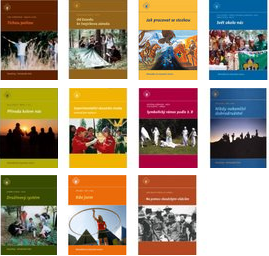
\includegraphics[height=1.25cm]{prirucky.png}
	\end{center}
\end{frame}

\subsection{Zdroje informací}

\begin{frame}[allowframebreaks]{Další informace}
	\begin{itemize}
		\item Informace o~skautském výchovném programu: \url{https://krizovatka.skaut.cz/vedu-oddil/skautska-vychova}
		\begin{itemize}
			\item Materiály ke~stažení
			\item Informace o~seminářích, kurzech,~\ldots
			\item Databáze programů
			\item Řada dalších informací\ldots
			\item Vše o~stezce: \url{https://stezka.skaut.cz/}
		\end{itemize}
		\item Web pro veřejnost: \url{https://www.skaut.cz/}
		\item Časopisy a~další materiály elektronicky: \url{https://casopisy.skaut.cz/}
		\item Knihy \textbf{Skautské století} (Roman Šantora, Václav Nosek, Slavomil Janov a~Václav Dostál, TDC a~Mladá fronta, 2012), \textbf{Skautský oddíl 1913--2013} (Roman Šantora a~kol., TDC a~Mladá fronta, 2014) a~\href{https://www.junshop.cz/knihy}{další}\ldots
		\item Skautský institut: \url{https://www.skautskyinstitut.cz/} (vzdělávání, historie skautingu, akce pro veřejnost)
		\item Aktuálně\ldots
		\begin{itemize}
			\item \textbf{Zpravodajství} \url{https://zpravodajstvi.skaut.cz/}
			\item \href{https://krizovatka.skaut.cz/ukrajina}{Pomoc ukrajinským uprchlíkům}, zapojení ukrajinských dětí do~oddílů
			\item \href{https://krizovatka.skaut.cz/klimaticka-zmena/rozcestnik-ke-klimaticke-zmene}{Rozcestník ke~klimatické změně}
		\end{itemize}
		\item Junák nabízí poradnu týkající se různých výchovných témat, personalistiky apod., \url{https://krizovatka.skaut.cz/vedeni-strediska/zpravodajove-pro-personalistiku/kontakt}
		\item Budete-li mít v~budoucnu dotazy, klidně se~mi ozvěte a~zeptejte se, \url{https://trapa.cz/cs/contact}
	\end{itemize}
\end{frame}

\begin{frame}{Děkuji za~pozornost\ldots}
	\begin{center}
		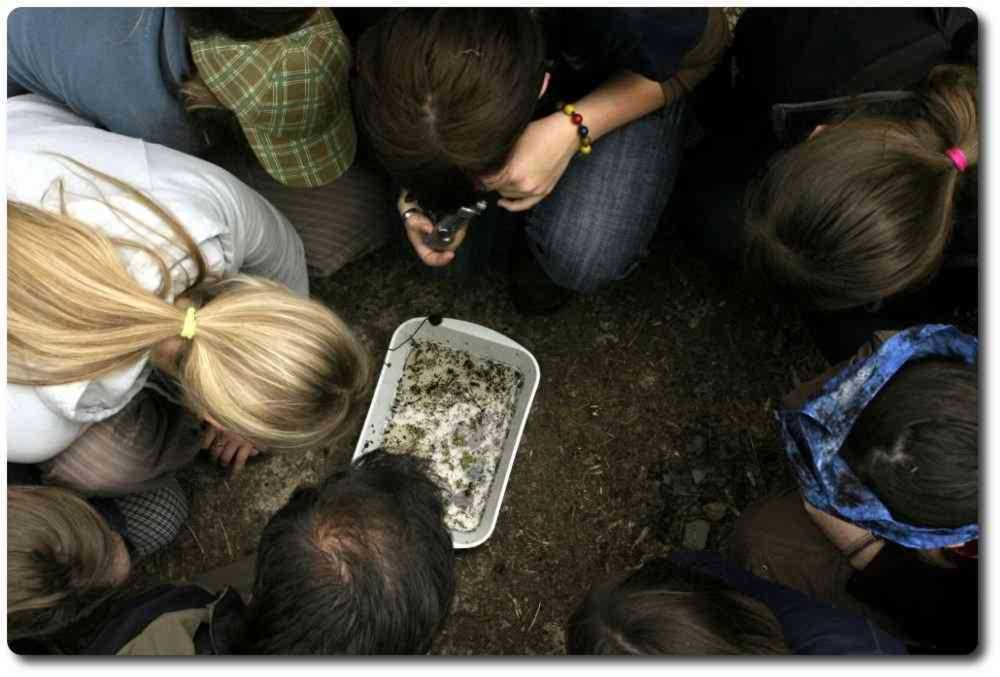
\includegraphics[height=6cm]{zaver.jpg}
	\end{center}
	\begin{flushright}
		\begin{large}
			\ldots otázky?
		\end{large}
	\end{flushright}
\end{frame}

\end{document}
